% Author: Izaak Neutelings (October 2021)
% Inspiration:
%  "Spacetime and Geometry: An Introduction to General Relativity", Sean M. Carroll
%  "Gravity: An Introduction to Einstein's General Relativity", James B. Hartle
\documentclass[border=3pt,tikz]{standalone}
\usepackage{tikz}
\usepackage{amsmath} % for \text
\usepackage{mathrsfs} % for \mathscr
\usepackage{xfp} % higher precision (16 digits?)
\usepackage[outline]{contour} % glow around text
\usetikzlibrary{decorations.markings,decorations.pathmorphing}
\usetikzlibrary{arrows.meta} % for arrow size
\contourlength{1.2pt}

\newcommand{\calI}{\mathscr{I}} %\mathcal
\tikzset{>=latex} % for LaTeX arrow head
\colorlet{myred}{red!80!black}
\colorlet{myblue}{blue!80!black}
\colorlet{mygreen}{green!80!black}
\colorlet{mydarkred}{red!50!black}
\colorlet{mydarkblue}{blue!50!black}
\colorlet{mylightblue}{mydarkblue!6}
\colorlet{mypurple}{blue!40!red!80!black}
\colorlet{mydarkpurple}{blue!40!red!50!black}
\colorlet{mylightpurple}{mydarkpurple!80!red!6}
\colorlet{myorange}{orange!40!yellow!95!black}
\tikzstyle{cone}=[mydarkblue,line width=0.2,top color=blue!60!black!30,
                  bottom color=blue!60!black!50!red!30,shading angle=60,fill opacity=0.9]
\tikzstyle{cone back}=[mydarkblue,line width=0.1,dash pattern=on 1pt off 1pt]
\tikzstyle{world line}=[myblue!60,line width=0.4,shorten <=-2mm,shorten >=-2mm]
\tikzstyle{world line t}=[mypurple!60,line width=0.4,shorten <=-2mm,shorten >=-2mm]
\tikzstyle{particle}=[mygreen,line width=0.5]
\tikzstyle{photon}=[-{Latex[length=4,width=3]},myorange,line width=0.4,decorate,
                    decoration={snake,amplitude=0.9,segment length=4,post length=3.8}]
\tikzstyle{singularity}=[myred,line width=0.6,decorate,
                         decoration={zigzag,amplitude=1.8,segment length=5}]
\tikzset{declare function={% Kruskal-Szekeres coordinates
  sing(\x)        = {\fpeval{sqrt(\x*\x+1)}};%
  rstar(\c)       = {\fpeval{(\c/2-1)*exp(\c/2)}};%
  kruskalu(\x,\c) = {\fpeval{sqrt(\x*\x+(\c/2-1)*exp(\c/2))}};%
  kruskalv(\x,\c) = {\fpeval{sqrt(\x*\x-(\c/2-1)*exp(\c/2))}};%
}}
\def\tick#1#2{\draw[thick] (#1) ++ (#2:0.04) --++ (#2-180:0.08)}
\def\Nsamples{50} % number samples in plot

% HORIZON, r=2M
\def\rtinf#1{\color{mydarkblue}
  r &\color{mydarkblue}= 2M \\[-2mm] \color{mydarkpurple}
  t &\color{mydarkpurple}= #1\infty \color{black}
}

% LIGHTCONE
\def\R{0.10} % size lightcone
\def\e{0.08} % vertical scale
\def\ang{45} % angle light cone
\def\angb{acos(sqrt(\e)*sin(\ang))} % angle ellipse center to point of tangency
\def\a{\R*sin(\ang)*sqrt(1-\e*sin(\ang)^2)/(1-\e*sin(\ang)^2)} % vertical radius
\def\b{\R*sqrt(\e)*sin(\ang)*cos(\ang)/(1-\e*sin(\ang)^2)} % horizontal radius
\def\coneback#1{ % light cone part to be drawn behind world lines
  \draw[cone back] % dashed line back
    (#1)++(-45:\R) arc({90-\angb}:{90+\angb}:{\a} and {\b});
  \draw[cone,shading angle=-60] % top edge & inside
    (#1)++(0,{\R*cos(\ang)/(1-\e*sin(\ang)^2)}) ellipse({\a} and {\b});
}
\def\conefront#1{ % light cone part to be drawn over world lines
  \draw[cone] % light cone outside
    (#1) --++ (45:\R) arc({\angb-90}:{-90-\angb}:{\a} and {\b})
     --++ (-45:2*\R) arc({90-\angb}:{-270+\angb}:{\a} and {\b}) -- cycle;
}

\begin{document}



% KRUSKAL DIAGRAM - equidistant world lines
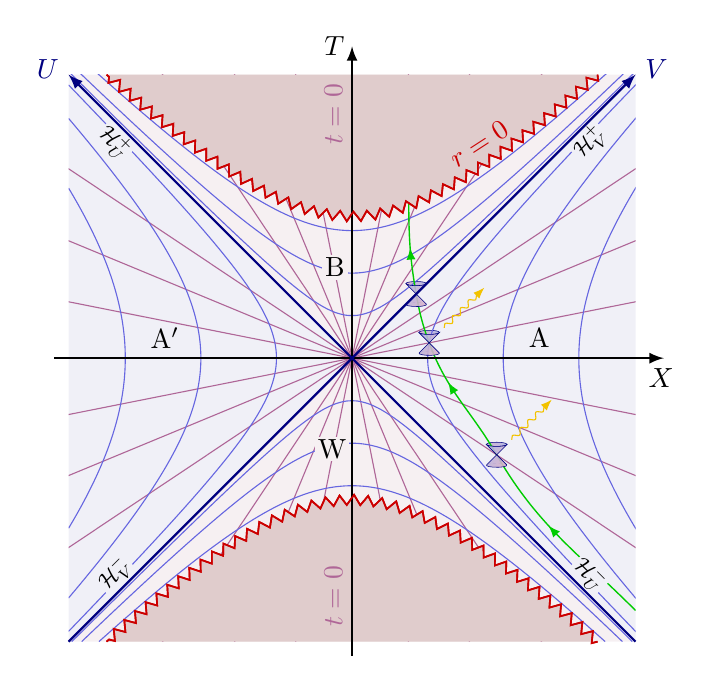
\begin{tikzpicture}[scale=1.8]
  \message{Kruskal diagram^^J}
  
  \def\xmax{2}
  \def\Nlines{3} % number of world lines (at constant r/t)
  \pgfmathsetmacro\ta{tan(45/(\Nlines+1))} % constant t value 1
  \pgfmathsetmacro\ra{(1.6/\Nlines)} % constant r value 1
  \coordinate (O)  at ( 0, 0); % center I: origin (r,t) = (0,0)
  \coordinate (SW) at (-\xmax,-\xmax); % horizon r=2M, t=-infty, region I
  \coordinate (SE) at ( \xmax,-\xmax); % horizon r=2M, t=-infty, region I
  \coordinate (NW) at (-\xmax, \xmax); % horizon r=2M, t=+infty, region IV
  \coordinate (NE) at ( \xmax, \xmax); % horizon r=2M, t=+infty, region IV
  \coordinate (X0) at (\xmax,-0.89*\xmax);
  \coordinate (X1) at ({0.51*\xmax},{-tan(135/(\Nlines+1))*0.51*\xmax});
  \coordinate (X2)  at ({\ra/sqrt(1-\ta*\ta)},{\ta*\ra/sqrt(1-\ta*\ta)});
  \coordinate (X3) at (45:0.32*\xmax); % particle falling in BH horizon
  \coordinate (X4)  at (0.2*\xmax,{sqrt((0.2*\xmax)^2+1.1)}); % particle falling in BH singularity
  
  % REGIONS FILLS
  \fill[mylightpurple] (NW) -- (O) -- (NE) -- cycle; % region I
  \fill[mylightblue]   (NE) -- (O) -- (SE) -- cycle; % region II
  \fill[mylightpurple] (SW) -- (O) -- (SE) -- cycle; % region III
  \fill[mylightblue]   (NW) -- (O) -- (SW) -- cycle; % region IV
  
  % LIGHT CONE BACK
  \coneback{X1};
  \coneback{X2};
  \coneback{X3};
  
  \begin{scope}
    \clip (-\xmax,-\xmax) rectangle (\xmax,\xmax);
    
    % CONSTANT T WORLD LINES
    \message{Making world constant-r lines (region I, III)...^^J}
    \foreach \i [evaluate={\ang=45*\i/(\Nlines+1); \y=tan(\ang)*\xmax}] in {1,...,\Nlines}{
      \message{  Running i/N=\i/\Nlines, ang=\ang...^^J}
      \draw[world line t] (-\xmax,-\y) -- ( \xmax,\y);
      \draw[world line t] ( \xmax,-\y) -- (-\xmax,\y);
      \draw[world line t] (-\y,-\xmax) -- ( \y,\xmax);
      \draw[world line t] ( \y,-\xmax) -- (-\y,\xmax);
    }
    \node[world line t,right] at (\xmax,{\xmax*tan(45/(\Nlines+1))}) {$t=\text{constant}$};
    \node[world line,above=2,right] at (\xmax,{kruskalv(\xmax,3)}) {$r=\text{constant}$};
    
    % CONSTANT R WORLD LINES
    \message{Making world constant-r lines (region I, III)...^^J}
    \foreach \i [evaluate={\c=1.6*\i/\Nlines; \vmax=sqrt(\xmax*\xmax-\c*\c);}] in {1,...,\Nlines}{
      \message{  Running i/N=\i/\Nlines, c=\c...^^J}
      \draw[world line,samples=\Nsamples,smooth,variable=\y,domain=-\vmax:\vmax]
        plot({-sqrt(\y*\y+\c*\c)},\y)
        plot({ sqrt(\y*\y+\c*\c)},\y);
    }
    \message{Making constant-r world lines (region II, IV)...^^J}
    \foreach \i [evaluate={\c=0.9*\i/\Nlines; \umax=sqrt(\xmax*\xmax-\c*\c);}] in {1,...,\Nlines}{
      \message{  Running i/N=\i/\Nlines, c=\c...^^J}
      \draw[world line,samples=\Nsamples,smooth,variable=\x,domain=-\umax:\umax]
        plot(\x,{-sqrt(\x*\x+\c*\c)})
        plot(\x,{ sqrt(\x*\x+\c*\c)});
    }
    
    % PARTICLE
    \draw[particle,decoration={markings,mark=at position 0.25 with {\arrow{latex}},
                                        mark=at position 0.61 with {\arrow{latex}},
                                        mark=at position 0.90 with {\arrow{latex}}},postaction={decorate}]
      (X0) to[out=135,in=-60] (X1) to[out=120,in=-70]
      (X2) to[out=110,in=-80] (X3) to[out=100,in=-90] (X4);
    
  \end{scope}
  
  % SINGULARITY
  \draw[singularity,fill=mydarkred!80!black!20,samples=\Nsamples,variable=\x, % singularity
        domain=sqrt(\xmax*\xmax-1):-sqrt(\xmax*\xmax-1)]
    plot(\x,{sqrt(\x*\x+1)});
  \draw[singularity,fill=mydarkred!80!black!20,samples=\Nsamples,variable=\x, % singularity
        domain=sqrt(\xmax*\xmax-1):-sqrt(\xmax*\xmax-1)]
    plot(\x,{-sqrt(\x*\x+1)});
  
  % LIGHT CONE FRONT
  \conefront{X1};
  \conefront{X2};
  \conefront{X3};
  
  % ESCAPING PHOTONS
  \draw[photon] (X1) ++ (45:0.15) --++ (45:0.4);
  \draw[photon] (X2) ++ (45:0.15) --++ (45:0.4);
  
  % LABELS
  \pgfmathsetmacro\rl{-0.26*\xmax} % r left
  \pgfmathsetmacro\rr{0.35*\xmax} % r right

  \node[myred,above right=1,rotate=33] at (\rr,{sqrt((\rr)^2+1)}) {$r=0$};
  \node[fill=mylightblue,inner sep=1,rotate=45,below left=0,scale=0.8] at (45:1.2*\xmax) {$\mathcal H^+_V$};
  \node[fill=mylightblue,inner sep=1,rotate=-45,below right=0,scale=0.8] at (135:1.2*\xmax) {$\mathcal H^+_U$};
  \node[fill=mylightblue,inner sep=1,rotate=-45,above left=0,scale=0.8] at (-45:1.2*\xmax) {$\mathcal H^-_U$};
  \node[fill=mylightblue,inner sep=1,rotate=45,above right=0,scale=0.8] at (-135:1.2*\xmax) {$\mathcal H^-_V$};

  \node[world line t,above=1,rotate=90] at (0,0.85*\xmax) {$t=0$};
  \node[world line t,above=1,rotate=90] at (0,-0.85*\xmax) {$t=0$};

  \node[above=2,left,mydarkblue] at (-\xmax,\xmax)
    {$U$};
  \node[above=2,right,mydarkblue] at (\xmax,\xmax)
    {$V$};
  
  % AXES
  \draw[->,thick] (-\xmax-0.1,0) -- (\xmax+0.2,0) node[left=1,below] {$X$};
  \draw[->,thick] (0,-\xmax-0.1) -- (0,\xmax+0.2) node[left=-1] {$T$};
  \draw[singularity,samples=\Nsamples,variable=\x, % singularity
        domain=sqrt(\xmax*\xmax-1):-sqrt(\xmax*\xmax-1)]
    plot(\x,{sqrt(\x*\x+1)});
  \draw[singularity,samples=\Nsamples,variable=\x, % singularity
        domain=sqrt(\xmax*\xmax-1):-sqrt(\xmax*\xmax-1)]
    plot(\x,{-sqrt(\x*\x+1)});
  \draw[->,thick,mydarkblue] (SE) -- (O) -- (NW);
  \draw[->,thick,mydarkblue] (SW) -- (O) -- (NE);

  % REGIONS
  \node at (-0.66*\xmax,0.07*\xmax) {A$'$};
  \node at ( 0.66*\xmax,0.07*\xmax) {A};
  \node[fill=mylightpurple,inner sep=1] at (-0.06*\xmax,0.32*\xmax) {B};
  \node[fill=mylightpurple,inner sep=1] at (-0.07*\xmax,-0.32*\xmax) {W};
  
\end{tikzpicture}


\end{document}